\exercise{Statistics Refreshner}
\begin{questions}
	
	%----------------------------------------------
	\begin{question}{Expectation \& Variance}{8}		
	\begin{answer} 
			\begin{enumerate}
		\item We can define the expectation by \begin{equation}
 E \vert f \vert =    \sum\limits_{w \in\Omega }^{ }  P(w) f(w) 
\end{equation}
Which leads to the variance:
\begin{equation}
 var\left[ f \right] = E\left\lvert f^2 \right\rvert - E \left[ f \right]^2.
\end{equation}
 If we have 2 random variables X,Y and Z = X + Y. 
Then is the expectation a linear function, since for any 2 points 
\begin{equation}
E\left[ Z \right] = \sum\limits_{w \in\Omega }^{ }  Z(w) P(w)  = \sum\limits_{w \in\Omega }^{ } (X(w)+ Y(w))P(w) = E\left[ X \right] + E\left[ Y \right]
\end{equation}
applies. Since the variance of the sum of 2 random variables is 
\begin{equation}
var\left[ Z \right] = E\left[ Z^2 \right] - E\left[ Z \right]^2 = var\left\lvert X \right\rvert + var\left[ Y \right] + 2E\left[ XY \right] - 2E\left[ X \right]E\left[ Y \right] is E\left[ XY \right] \neq E\left[ X \right] E\left[ Y \right] 
\end{equation}
\begin{equation}
And that is not a linear operator.
\end{equation}

		\item Unbiased estimator: 
		\begin{equation}
		\overline{x} = \frac{1}{n} * \sum\limits_{i=1}^{n} {  x_{ i } }
		\end{equation}
				\begin{equation}
						\overline{xA} = \frac{ 1 }{  6} *(1 + 5 + 6 +3 +2 + 1) = 3
		\end{equation}
				\begin{equation}
						\overline{xB} =\frac{ 1 }{  6} *(6 + 1+ 1 + 4 + 1 + 5) = 3
		\end{equation}
				\begin{equation}
						\overline{xC} =  \frac{ 1 }{  6} *(3 + 2 + 3 + 3 +4 +3) = 3
		\end{equation}
		unbiased estimator for the variance
				\begin{equation}
				\overline{\sigma} = \frac{1}{n -1} * \sum\limits_{i=1}^{n} {  x_{ i }  - \overline{x}}^2
		\end{equation}
		\begin{equation}
		\overline{\sigma A}  = \frac{ 1 }{ 5 } * ((1 - 3)^2 + (5 - 3)^2 + (6 - 3)^2 + (3 - 3)^2 + (2 - 3)^2 + (1 - 3)^2) = \frac{ 22 }{  5} = 4,4
		\end{equation}
				\begin{equation}
		\overline{\sigma B} =\frac{ 1 }{  5} * ((6 - 3)^2 + (1 - 3)^2 + (1 - 3)^2 + (4 - 3)^2 + (1 - 3)^2 + (5 - 3)^2) = \frac{ 26 }{5  } = 5,2
		\end{equation}
				\begin{equation}
		\overline{\sigma C}  = \frac{ 1 }{ 5 }  * ((3 - 3)^2 + (2 - 3)^2 + (3 - 3)^2 + (4 - 3)^2 + (3 - 3)^2 + (3 - 3)^2) = \frac{ 2 }{ 5 } = 0,4
		\end{equation}
		
		
		\item
		\begin{equation}
		KL: \sum\limits_{x\in X}^{} {  P(x) ln \frac{ P(x) }{ Q(x) } }
		\end{equation}
		\begin{equation}
		KL(PA \parallel Q) = \frac{ 3 }{ 6 } * ln (\frac{ \frac{ 3 }{6  } }{ \frac{ 1 }{ 6 } }) + \frac{ 1 }{ 6 } * ln (\frac{ \frac{ 1}{6  } }{ \frac{ 1 }{ 6 } }) +  \frac{ 1 }{ 6 } * ln (\frac{ \frac{ 1}{6  } }{ \frac{ 1 }{ 6 } }) +  \frac{ 1 }{ 6 } * ln (\frac{ \frac{ 1}{6  } }{ \frac{ 1 }{ 6 } }) +  \frac{ 1 }{ 6 } * ln (\frac{ \frac{ 1}{6  } }{ \frac{ 1 }{ 6 } })  = 3
		\end{equation}
		
				\begin{equation}
		KL(PB \parallel Q) = \frac{ 1 }{ 6 } * ln (\frac{ \frac{ 1 }{6  } }{ \frac{ 1 }{ 6 } }) + \frac{ 2 }{ 6 } * ln (\frac{ \frac{ 2 }{6  } }{ \frac{ 1 }{ 6 } }) + \frac{ 1 }{ 6 } * ln (\frac{ \frac{ 1 }{6  } }{ \frac{ 1 }{ 6 } }) + \frac{ 1 }{ 6 } * ln (\frac{ \frac{ 1 }{6  } }{ \frac{ 1 }{ 6 } }) = 1,52
		\end{equation}
				\begin{equation}
		KL(PC\parallel Q) = \frac{ 4 }{ 6 } * ln (\frac{ \frac{ 4 }{6  } }{ \frac{ 1 }{ 6 } }) + \frac{ 1 }{ 6 } * ln (\frac{ \frac{ 1 }{6  } }{ \frac{ 1 }{ 6 } }) + \frac{ 1 }{ 6 } * ln (\frac{ \frac{ 1 }{6  } }{ \frac{ 1 }{ 6 } })  = 2.38
		\end{equation}
		A has the biggest KL divergence, so it is the closest
		\end{enumerate}
	\end{answer}
	\end{question}
	
	%----------------------------------------------	
	
	\begin{question}{It is a cold world}{7}		
	\begin{answer} 
	\begin{enumerate}
		\item 
			\begin{equation}
			a \in\left\{ 0, 1 \right\}: if a person has backspin, with 1 = pain and 0 = no pain
			\end{equation}
			\begin{equation}
			b \in\left\{ 0, 1 \right\}: if a person has a cold, with 1 = pain and 0 = no cold
			\end{equation}
		\item \begin{equation}
		P(a = 1 \mid b = 1) = 0,25
		\end{equation}
		\begin{equation}
		P( b = 1) = 0,04
		\end{equation}
		\begin{equation}
		P(a = 1 \mid b = 0) = 0,1
		\end{equation}
		\item Rule of Bayes
		\begin{equation}
		P(b = 1 \mid a = 1) =  \frac{ P(a = 1 \mid b = 1) P(b = 1) }{ P(b = 1)  }
		\end{equation}
				\begin{equation}
				\frac{ P(a = 1 \mid b = 1) P(b = 1) }{ P (a = 1 \mid b = 1) P (b = 1) + P(a = 1 \mid b = 0) P(b = 0 ) }
		\end{equation}
				\begin{equation}
				Werte einsetzen: \frac{ 0,25 * 0,04 }{0,25 * 0,04 + 0,10 * (1 - 0,04)  } = \frac{ 5 }{ 53 } \approx 0,094
		\end{equation}
		
		\end{enumerate}
		
	\end{answer}
		
	\end{question}

	%----------------------------------------------
	
\begin{question}{Cure the virus}{14}		
	\begin{answer} 
	\begin{enumerate}
		\item Markov Chain
				\begin{equation}
				S_{0} = 
\begin{pmatrix}
1 \\
0

\end{pmatrix}
		\end{equation}
						\begin{equation}
				S_{1} = 
\begin{pmatrix}
0,42 \\
0,58

\end{pmatrix}
		\end{equation}
		\begin{equation}
						P_{} = 
\begin{pmatrix}
0,42 & 0,974\\
0,58 & 0,026

\end{pmatrix}
		\end{equation}
		\begin{equation}
		S_{1} = P * S_{0} \leftrightarrow \begin{pmatrix}
0,42 \\
0,58

\end{pmatrix} = \begin{pmatrix}
0,42 & 0,974\\
0,58 & 0,026

\end{pmatrix} * \begin{pmatrix}
1 \\
0

\end{pmatrix}
		\end{equation}
		
			\begin{equation}
			S_{2} = P * S_{1} \leftrightarrow \begin{pmatrix}
0,741 \\
0,394 

\end{pmatrix} = \begin{pmatrix}
0,42 & 0,974\\
0,58 & 0,026

\end{pmatrix} * \begin{pmatrix}
0,42 \\
0,58

\end{pmatrix} 
		\end{equation}
		
		\item \lstinputlisting[language=Python]{virus_Task3.py}
		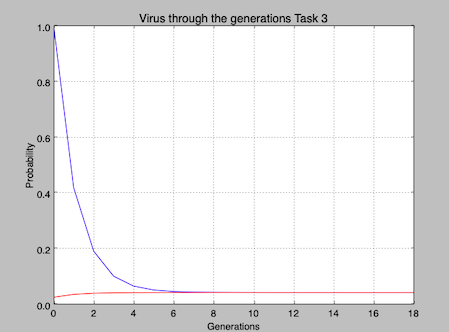
\includegraphics{plot_Markov}\\
		\item
		After 6 timesteps does the ratios stop to change significantly. Stable probability:
		\begin{equation}
								P_{} = 
\begin{pmatrix}
0,42 & 0,974\\
0,58 & 0,026

\end{pmatrix}
		\end{equation}
				\begin{equation}
								\overline{X} = 
\begin{pmatrix}
A\\
B

\end{pmatrix}
		\end{equation}
						\begin{equation}
								P* \overline{X} = \overline{X} \leftrightarrow \begin{pmatrix}
0,42 & 0,974\\
0,58 & 0,026

\end{pmatrix} * \begin{pmatrix}
A\\
B

\end{pmatrix} = \begin{pmatrix}
A\\
B

\end{pmatrix}
		\end{equation}
		\begin{equation}
		0,42 A + 0,5B = A \Rightarrow 0,5B = A - 0,42A 
		\Rightarrow B = \frac{ 25 }{ 29 } = 0,86
		\end{equation}
		
				\begin{equation}
				0,58A + 0,026B = B
		\end{equation}
				
		\begin{equation}
				A + B = 1 \Rightarrow  A + 0,86 = 1 \Rightarrow  A = 0,14
		\end{equation}
		We can see the probability converge to our solution.
		\end{enumerate}
	\end{answer}	
	\end{question}	
\end{questions}

